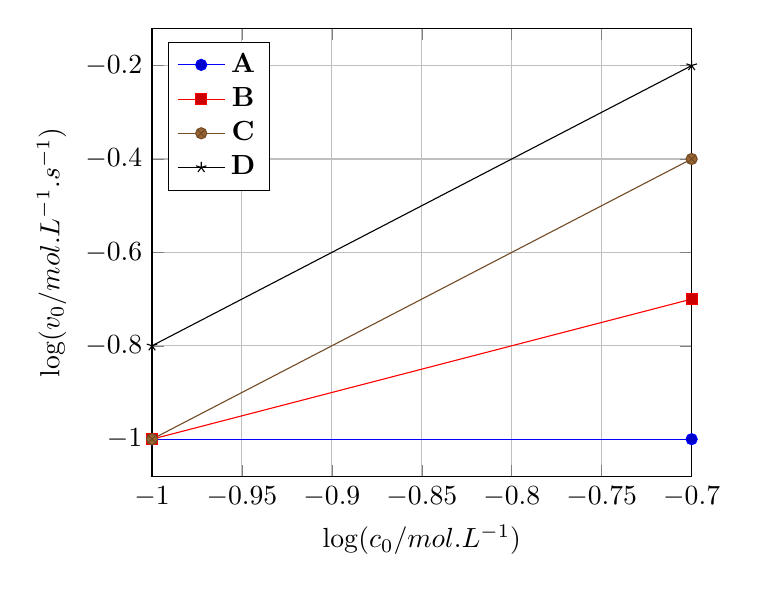
\begin{tikzpicture}
    \begin{axis}
        [
            legend pos = north west,
            xlabel = {$\log(c_0/\unit{mol.L^{-1}})$},
            ylabel = {$\log(v_0/\unit{mol.L^{-1}.s^{-1}})$},
            xmin = -1, xmax = -0.7,
            grid = major,
        ]
    \addplot coordinates
        {
            (  -1, -1)
            (-0.7, -1)
        };
    \addplot coordinates
        {
            (  -1,   -1)
            (-0.7, -0.7)
        };
    \addplot coordinates
        {
            (  -1,   -1)
            (-0.7, -0.4)
        };
    \addplot coordinates
        {
            (  -1, -0.8)
            (-0.7, -0.2)
        };
    \legend{\textbf{A}, \textbf{B}, \textbf{C}, \textbf{D}}
    \end{axis}
\end{tikzpicture}